%\VignetteIndexEntry{An Introduction to the Gifi package}
%\VignetteEngine{knitr::knitr} 
\documentclass[10pt,nojss,nofooter,fleqn]{jss}\usepackage[]{graphicx}\usepackage[]{color}
%% maxwidth is the original width if it is less than linewidth
%% otherwise use linewidth (to make sure the graphics do not exceed the margin)
\makeatletter
\def\maxwidth{ %
  \ifdim\Gin@nat@width>\linewidth
    \linewidth
  \else
    \Gin@nat@width
  \fi
}
\makeatother

\definecolor{fgcolor}{rgb}{0.345, 0.345, 0.345}
\newcommand{\hlnum}[1]{\textcolor[rgb]{0.686,0.059,0.569}{#1}}%
\newcommand{\hlstr}[1]{\textcolor[rgb]{0.192,0.494,0.8}{#1}}%
\newcommand{\hlcom}[1]{\textcolor[rgb]{0.678,0.584,0.686}{\textit{#1}}}%
\newcommand{\hlopt}[1]{\textcolor[rgb]{0,0,0}{#1}}%
\newcommand{\hlstd}[1]{\textcolor[rgb]{0.345,0.345,0.345}{#1}}%
\newcommand{\hlkwa}[1]{\textcolor[rgb]{0.161,0.373,0.58}{\textbf{#1}}}%
\newcommand{\hlkwb}[1]{\textcolor[rgb]{0.69,0.353,0.396}{#1}}%
\newcommand{\hlkwc}[1]{\textcolor[rgb]{0.333,0.667,0.333}{#1}}%
\newcommand{\hlkwd}[1]{\textcolor[rgb]{0.737,0.353,0.396}{\textbf{#1}}}%

\usepackage{framed}
\makeatletter
\newenvironment{kframe}{%
 \def\at@end@of@kframe{}%
 \ifinner\ifhmode%
  \def\at@end@of@kframe{\end{minipage}}%
  \begin{minipage}{\columnwidth}%
 \fi\fi%
 \def\FrameCommand##1{\hskip\@totalleftmargin \hskip-\fboxsep
 \colorbox{shadecolor}{##1}\hskip-\fboxsep
     % There is no \\@totalrightmargin, so:
     \hskip-\linewidth \hskip-\@totalleftmargin \hskip\columnwidth}%
 \MakeFramed {\advance\hsize-\width
   \@totalleftmargin\z@ \linewidth\hsize
   \@setminipage}}%
 {\par\unskip\endMakeFramed%
 \at@end@of@kframe}
\makeatother

\definecolor{shadecolor}{rgb}{.97, .97, .97}
\definecolor{messagecolor}{rgb}{0, 0, 0}
\definecolor{warningcolor}{rgb}{1, 0, 1}
\definecolor{errorcolor}{rgb}{1, 0, 0}
\newenvironment{knitrout}{}{} % an empty environment to be redefined in TeX

\usepackage{alltt}
\usepackage{amsmath, amsfonts}
\usepackage{float,amssymb}
\usepackage{hyperref}

\newcommand{\defi}{\mathop{=}\limits^{\Delta}}  
%%%%%%%%%%%%%%%%%%%%%%%%%%%%%%
%% declarations for jss.cls %%%%%%%%%%%%%%%%%%%%%%%%%%%%%%%%%%%%%%%%%%
%%%%%%%%%%%%%%%%%%%%%%%%%%%%%%

%% almost as usual
\author{Patrick Mair \\ Harvard University \And 
        Jan de Leeuw \\ University of California, Los Angeles \AND
        Patrick Groenen \\ Erasmus University Rotterdam
}
\title{The Gifi Package for Categorical Multivariate Analysis in \proglang{R}}
%
%%% for pretty printing and a nice hypersummary also set:
\Plainauthor{Patrick Mair, Jan de Leeuw} %% comma-separated
\Plaintitle{Gifi Methods for Optimal Scaling in R: The Package homals} %% without formatting
\Shorttitle{Gifi in \proglang{R}} %% a short title (if necessary)

%% an abstract and keywords
\Abstract{
This package vignette is an update and extension of the paper by published in the Journal of Statistical Software.
Homogeneity analysis combines the idea of maximizing the correlations between variables of a multivariate data set with
that of optimal scaling. In this article we present methodological and practical issues of the \proglang{R} package \pkg{homals} which performs homogeneity analysis and various extensions. By setting rank constraints nonlinear principal component analysis can be performed. The variables can be partitioned into sets such that homogeneity analysis is extended to nonlinear canonical correlation analysis or to predictive models which emulate discriminant analysis and regression models. For each model the scale level of the variables can be taken into account by setting level constraints. All algorithms allow for missing values.
}
\Keywords{Gifi methods, optimal scaling, homogeneity analysis, correspondence analysis, nonlinear principal component analysis, nonlinear canonical correlation analysis, homals, \proglang{R}}
\Plainkeywords{Gifi methods, optimal scaling, homogeneity analysis, optimal scaling, correspondence analysis, nonlinear principal component analysis, nonlinear canonical correlation analysis, homals, R} %% without formatting
%% at least one keyword must be supplied

%% publication information
%% NOTE: This needs to filled out ONLY IF THE PAPER WAS ACCEPTED.
%% If it was not (yet) accepted, leave them commented.
%% \Volume{13}
%% \Issue{9}
%% \Month{September}
%% \Year{2004}
%% \Submitdate{2004-09-29}
%% \Acceptdate{2004-09-29}

%% The address of (at least) one author should be given
%% in the following format:
\Address{
  Patrick Mair\
  Department of Psychology\\
  Harvard University\\
  E-mail: \email{mair@fas.harvard.edu}\\
  URL: \url{http://scholar.harvard.edu/mair}
}
%% It is also possible to add a telephone and fax number
%% before the e-mail in the following format:
%% Telephone: +43/1/31336-5053
%% Fax: +43/1/31336-734

%% for those who use Sweave please include the following line (with % symbols):
%% need no \usepackage{Sweave.sty}

%% end of declarations %%%%%%%%%%%%%%%%%%%%%%%%%%%%%%%%%%%%%%%%%%%%%%%
\IfFileExists{upquote.sty}{\usepackage{upquote}}{}
\begin{document}



\section{Introduction}
\label{sec:int}


\section{Gifi Methods for Categorical Multivariate Analysis}
\label{sec:gifi}

\subsection{The Gifi Loss Function}
In this section we give the very general definition of the Gifi loss function. 
We restrict our elaborations to the very basic expressions. For simplicity, we are not incorporating the formulation for missing data even though the package allows for this. A more detailed and slightly more technical formulation can be found in \citet{deLeeuw+Mair:2009a}. 


Homogeneity analysis is based on the criterion of minimizing the departure from homogeneity. This departure is measured by a loss function. To write the corresponding basic equations the following definitions are needed. For $i=1,\ldots,n$ objects, data on $m$ (categorical) variables are collected where each of the $j=1,\ldots,m$ variable takes on $k_j$ different values (their \emph{levels} or \emph{categories}). We code them using $n\times k_j$ binary \emph{indicator matrices} $G_j$, i.e., a matrix of dummy variables for each variable. The whole set of indicator matrices can be collected in a block matrix
\begin{equation}
G\defi\begin{bmatrix}G_1&\vdots&G_2&\vdots&\cdots&\vdots&G_m\end{bmatrix}.
\end{equation}
For convenience we introduce $D_j^{}=G_j'G_j^{}$ as the $k_j\times k_j$ diagonal matrix with the (marginal) frequencies of variable $j$ in its main diagonal. 

Let $X$ be the unknown $n\times p$ matrix containing the coordinates (\emph{object scores}) of the object projections into $\mathbb{R}^p$. Furthermore, let $Y_j$ be the unknown $k_j \times p$ matrix containing the coordinates of the category projections into the same $p$-dimensional space (\emph{category quantifications}). 
The problem of finding these solutions can be formulated by means of the following loss function to be minimized:
\begin{equation}
\label{eq:loss}
\sigma(X;Y_1,\ldots,Y_m) = \frac{1}{m} \sum_{j=1}^m\mathbf{tr}(X-G_jY_j)'(X-G_jY_j)
\end{equation}
We use the normalization $X'X=I$ in order to avoid the trivial solution $X=0$ and $Y_j=0$. Note that from an analytical point of view the loss function represents the sum-of-squares of $(X-G_jY_j)$ which obviously involves the object scores and the category quantifications. Thus, we minimize simultaneously over $X$ and $Y_j$. 

This minimization problem is solved by the iterative \emph{alternating least squares algorithm} (ALS; sometimes quoted as \emph{reciprocal averaging algorithm}). At iteration $t=0$ we start with arbitrary object scores $X^{(0)}$. Each iteration $t$ consists of three steps:
\begin{enumerate}
\item Update category quantifications: $Y_j^{(t+1)}=D_j^{-1}G_j'X^{(t)}$ for $j=1,\ldots,m$
\item Update object scores: $\tilde X^{(t+1)}=\sum_{j=1}^m G_j^{}Y_j^{(t+1)}$
\item Normalization: $X^{(t+1)}= \sqrt{n}\tilde X^{(t+1)}\left(\tilde X^{(t+1)}{'}\tilde X^{(t+1)}\right)^{-\frac{1}{2}}$
\end{enumerate}
The algorithm stops when the decrease in the loss function gets below a prespecified level $\varepsilon$. 

These are the ingredients we need in order to formulate important variants of the general Gifi model. 
In the following section we start with the most important one: PRINCALS.

\section{Categorical Principal Component Analysis}
\label{sec:princals}
Standard PCA was developed for metric variables and assumes that the relationships between the variables are linear. PCA aims to 
explain variance. It can be solved by an eigenvalue decomposition of the corresponding correlation (or covariance) matrix: the eigenvalues represent the variances of the principal component scores and the eigenvectors give the vectors of weights (loadings). PCA is targeted on explaining variance and typically we are aiming to find a satisfactory solution (in terms of the explained amount of variance) in a low-dimensional space. 

From a homogeneity analysis perspective, the PCA problem can be stated as follows: 


In many fields researchers often have to deal with categorical variables such as Likert items in the Social Sciences. Running a PCA on a set of items implies treating them as metric, i.e. the distances between categories (i.e. 1--2, 2--3, 3--4, etc.) have to be constant across categories. Together with the linear relationship assumption, these requirements are often not fulfilled in practice. 
In addition, the concept of variance only applied to metric variables. 

If we want to treat the variables on an ordinal scale, we have two options: run an ordinal factor analysis (FA) based on polychoric correlations as implemented in the \code{fa.poly()} function in the \pkg{psych} package, or run a categorical (ordinal) PCA as presented here. Apart from the conceptual differences between FA and PCA, the advantage of PRINCALS over polychoric FA is that we do not have to pose any underlying distribution assumption on our data, whereas a polychoric (or tetrachoric in the binary case) correlation assumes that the categories are realizations of an underlying latent normal distribution. 

PRINCALS does not only allow for ordinal input data, it can be also applied to mixed scale levels: some variables can be metric, 
some variables ordinal, some variables nominal. 



In \pkg{homals} there is the \code{princals()} function which performs NLPCA. Since NLPCA is just a rank-1 restricted 
version of general homogeneity analysis, internally \code{princals()} uses \code{homals()} as engine. An effort was made 
to make the PRINCALS output as PCA-like (i.e. \code{princomp()}-like) as possible in terms of comparable 
eigenvalues, explaned amount of variance on each dimension, and loadings.

Standard PCA is solved by an eigenvalue decomposition of the input correlation matrix $R$ based on the original 
data which gives us eigenvalue vector $\lambda$ of length $m$. Subsequently, the amount 
of explained variance for each dimension can be computed by dividing each eigenvalue by the sum of the $m$ eigenvalues. 
One of the cores outputs of any Gifi model is that it provides a ``new'' data matrix where the original categories are optimally scaled for each dimension. Now can now compute the correlation matrix $R^{\ast}$ on the new data matrix (it does not matter 
which one we use since the $p$ matrices are linearly dependent) and perform an eigenvalue decomposition. 
This gives us the eigenvalue vector $\lambda^{\ast}$ of length $m$. As above, we can compute the amount 
of explained variance for each of the $m$ dimensions. In addition, in order to evaluate the amount of ``improvement'' 
of NLPCA over PCA we can compute the eigenvalue ratio, e.g. for the first dimension we have $\lambda_1^{\ast}/\lambda_1$. 
This gives us a measure for the violations of equidistance and linearity in our original data. 

Regarding the loadings, in standard PCA they are normed to $\|w\|^2 = 1$. 
In order to make the loadings $w^{\ast}$ from NLPCA comparable to standard PCA, they need to be normalized the same way.
The \code{princals()} function performs all these computations internally and returns the $p$ eigenvalues based on the 
$R^{\ast}$, the amount of variance explained for each of the $p$ dimensions, and the standardized loadings. 

Through the \code{level} argument the user can specify the scale levels of the variables (\code{"ordinal" as default}. If all variables are set to \code{"numerical"}, PRINCALS mimics standard PCA. In terms of plotting possibilities, a generic plot function allows for a loadings plot (default), a scree plot, transformation plots, and a biplot by specifying the 
\code{plot.type} argument accordingly. 

\subsection{Rotation and Goodness-Of-Fit}
The package also offers options for rotating a PRINCALS solution. Note that ``rotation'' is a concept developed within factor 
analysis (FA) by transforming the factor loadings through a rotation matrix and computing the corresponding rotated factor scores 
afterwards. Strictly speaking, PCA eigenvectors of the correlation/covariance matrix are not loadings (even though we just called them ``loadings'') above. Loadings within an FA context are eigenvectors scaled by the square roots of the corresponding eigenvalues. 
For unrotated PCA/PRINCALS solutions this difference is not so important, but if we want to rotate a solution the PCA/PRINCALS 
``loadings'' need to be re-scaled such that they are loadings in the FA sense. Thus, we can apply standard \code{varimax()} and \code{promax()} rotations as provided in \pkg{stats}. In order to get the rotated principal scores, we multiply unrotated matrix 
of the PRINCALS PC-scores with the generalized inverse of the rotated loadings matrix. 


\subsection{Example: ABC Company}
Now we show an ordinal PCA example on the ABC dataset which reproduces the analysis in \cite{Ferrari+Barbiero:2012}. 
ABC is a ficticious company which launched a customer satisfaction survey. In this analysis we use six items, 
each of them on a 5-point Likert scale, covering certain aspects of customer satisfaction: 
equipment, sales support, technical support, training, purchase, and pricing. 

First, we start with a full-dimensional PRINCALS solution and examine the scree plot.

\begin{knitrout}
\definecolor{shadecolor}{rgb}{0.969, 0.969, 0.969}\color{fgcolor}\begin{kframe}
\begin{alltt}
\hlstd{ABC6} \hlkwb{<-} \hlstd{ABC[,} \hlnum{6}\hlopt{:}\hlnum{11}\hlstd{]}
\hlstd{fitfull} \hlkwb{<-} \hlkwd{princals}\hlstd{(ABC6,} \hlkwc{ndim} \hlstd{=} \hlnum{6}\hlstd{)}
\hlstd{fitfull}
\end{alltt}
\begin{verbatim}
## Call: princals(data = ABC6, ndim = 6)
## 
## Loss: 0.000667735
## Number of iterations: 19 
## 
## Eigenvalues:
##  Comp.1  Comp.2  Comp.3  Comp.4  Comp.5  Comp.6 
## 2.31083 1.00248 0.76242 0.73749 0.67682 0.50996
\end{verbatim}
\begin{alltt}
\hlkwd{summary}\hlstd{(fitfull)}
\end{alltt}
\begin{verbatim}
## 
## Loadings: 
##           Comp.1 Comp.2 Comp.3 Comp.4 Comp.5 Comp.6
## equipment  0.275 -0.744 -0.371 -0.411  0.243  0.003
## sales      0.458 -0.091  0.504 -0.252 -0.438  0.517
## technical  0.409  0.035 -0.611  0.455 -0.508  0.025
## training   0.443  0.273 -0.043  0.266  0.695  0.422
## purchase   0.361  0.567 -0.190 -0.623 -0.022 -0.349
## pricing    0.469 -0.199  0.445  0.318  0.089 -0.658
## 
## Variance accounted for:
##                    Comp.1 Comp.2 Comp.3 Comp.4 Comp.5 Comp.6
## VAF (%)             38.51  16.71  12.71  12.29  11.28    8.5
## Cumulative VAF (%)  38.51  55.22  67.93  80.22  91.50  100.0
\end{verbatim}
\end{kframe}
\end{knitrout}

The scree plot is given in in the left panel of Figure \ref{fig:abcsree}. 

Second, we fit a two-dimensional ordinal solution. The loadings plot is given in Figure \ref{fig:abcscree} (right panel). 
\begin{knitrout}
\definecolor{shadecolor}{rgb}{0.969, 0.969, 0.969}\color{fgcolor}\begin{kframe}
\begin{alltt}
\hlstd{fit2d} \hlkwb{<-} \hlkwd{princals}\hlstd{(ABC6,} \hlkwc{ndim} \hlstd{=} \hlnum{2}\hlstd{)}
\hlstd{fit2d}
\end{alltt}
\begin{verbatim}
## Call: princals(data = ABC6, ndim = 2)
## 
## Loss: 0.0005475663
## Number of iterations: 38 
## 
## Eigenvalues:
##  Comp.1  Comp.2 
## 2.94546 0.85430
\end{verbatim}
\begin{alltt}
\hlkwd{summary}\hlstd{(fit2d)}
\end{alltt}
\begin{verbatim}
## 
## Loadings: 
##           Comp.1 Comp.2
## equipment  0.456 -0.032
## sales      0.374 -0.652
## technical  0.392  0.326
## training   0.393  0.491
## purchase   0.397  0.270
## pricing    0.432 -0.393
## 
## Variance accounted for:
##                    Comp.1 Comp.2
## VAF (%)             49.09  14.24
## Cumulative VAF (%)  49.09  63.33
\end{verbatim}
\end{kframe}
\end{knitrout}
We see that we explain around 63\% of the variance.

\begin{knitrout}
\definecolor{shadecolor}{rgb}{0.969, 0.969, 0.969}\color{fgcolor}\begin{kframe}
\begin{alltt}
\hlstd{op} \hlkwb{<-} \hlkwd{par}\hlstd{(}\hlkwc{mfrow} \hlstd{=} \hlkwd{c}\hlstd{(}\hlnum{1}\hlstd{,}\hlnum{2}\hlstd{))}
\hlkwd{plot}\hlstd{(fitfull,} \hlkwc{plot.type} \hlstd{=} \hlstr{"screeplot"}\hlstd{)}
\hlkwd{plot}\hlstd{(fit2d)}
\hlkwd{par}\hlstd{(op)}
\end{alltt}
\end{kframe}
\end{knitrout}
\begin{figure}
\begin{center}  % fig.width='15cm', fig.height='6cm'
\begin{knitrout}
\definecolor{shadecolor}{rgb}{0.969, 0.969, 0.969}\color{fgcolor}
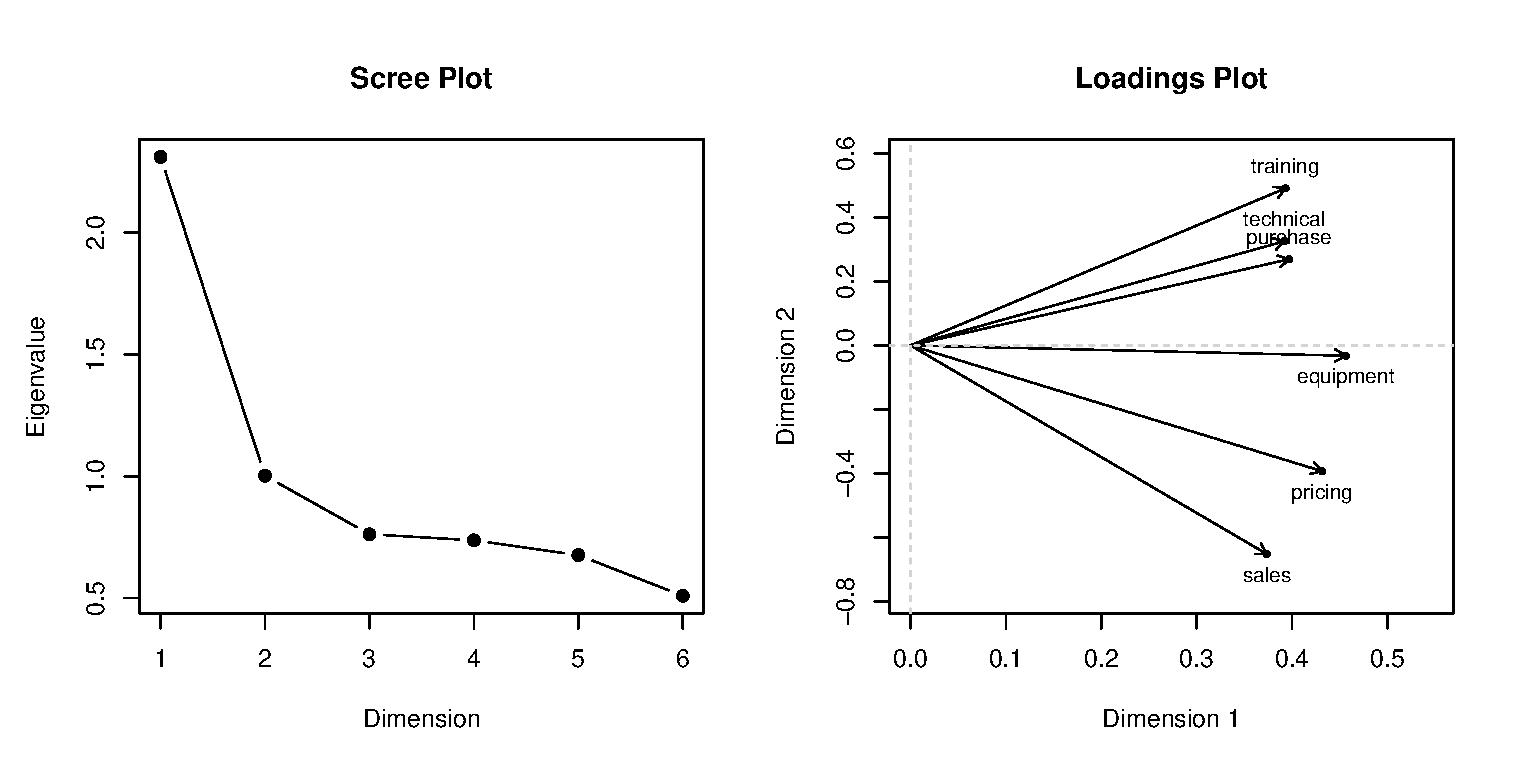
\includegraphics[width=\maxwidth]{figure/abcscree-plot1-1} 

\end{knitrout}
\end{center}
\caption{\label{fig:abcscree} Left panel: Scree plot for full-dimensional PRINCALS. Right panel: 
Loadings plot for two-dimensional solution.}
\end{figure}

Now we fit a one-dimensional ordinal PCA.
\begin{knitrout}
\definecolor{shadecolor}{rgb}{0.969, 0.969, 0.969}\color{fgcolor}\begin{kframe}
\begin{alltt}
\hlstd{fit1d} \hlkwb{<-} \hlkwd{princals}\hlstd{(ABC6,} \hlkwc{ndim} \hlstd{=} \hlnum{1}\hlstd{)}
\hlstd{fit1d}
\end{alltt}
\begin{verbatim}
## Call: princals(data = ABC6, ndim = 1)
## 
## Loss: 0.0004027625
## Number of iterations: 10 
## 
## Eigenvalues:
##  Comp.1 
## 2.98414
\end{verbatim}
\begin{alltt}
\hlkwd{summary}\hlstd{(fit1d)}
\end{alltt}
\begin{verbatim}
## 
## Loadings: 
##           Comp.1
## equipment  0.448
## sales      0.387
## technical  0.390
## training   0.395
## purchase   0.396
## pricing    0.428
## 
## Variance accounted for:
##                    Comp.1
## VAF (%)             49.74
## Cumulative VAF (%)  49.74
\end{verbatim}
\end{kframe}
\end{knitrout}

Let us compare it with the outcome of a standard PCA solution using \code{princomp()} and compute the ratio of the first 
eigenvalues.

\begin{knitrout}
\definecolor{shadecolor}{rgb}{0.969, 0.969, 0.969}\color{fgcolor}\begin{kframe}
\begin{alltt}
\hlstd{ABC6m} \hlkwb{<-} \hlkwd{sapply}\hlstd{(ABC6,} \hlkwa{function}\hlstd{(}\hlkwc{x}\hlstd{)} \hlkwd{as.numeric}\hlstd{(}\hlkwd{levels}\hlstd{(x))[x])}
\hlstd{fitpc} \hlkwb{<-} \hlkwd{princomp}\hlstd{(ABC6m)}
\hlstd{fitpc}
\end{alltt}
\begin{verbatim}
## Call:
## princomp(x = ABC6m)
## 
## Standard deviations:
##    Comp.1    Comp.2    Comp.3    Comp.4    Comp.5    Comp.6 
## 1.6732946 0.9832548 0.8268262 0.7708195 0.6209486 0.5968660 
## 
##  6  variables and  208 observations.
\end{verbatim}
\begin{alltt}
\hlstd{fit1d}\hlopt{$}\hlstd{eigenvalues}\hlopt{/}\hlstd{(fitpc}\hlopt{$}\hlstd{sdev}\hlopt{^}\hlnum{2}\hlstd{)[}\hlnum{1}\hlstd{]}       \hlcom{## eigenvalue ratio NLPCA/PCA}
\end{alltt}
\begin{verbatim}
##   Comp.1 
## 1.065798
\end{verbatim}
\end{kframe}
\end{knitrout}

The eigenvalue ratio of suggests 1.07 a slight improvement 
of NLPCA over standard PCA. This implies that the response categories are approximately equidistant and 
the relationship between the variables is not far from linear.
If we want to mimic standard PCA with PRINCALS, we declare all the variables as numeric.

\begin{knitrout}
\definecolor{shadecolor}{rgb}{0.969, 0.969, 0.969}\color{fgcolor}\begin{kframe}
\begin{alltt}
\hlstd{fit1dm} \hlkwb{<-} \hlkwd{princals}\hlstd{(ABC6,} \hlkwc{ndim} \hlstd{=} \hlnum{1}\hlstd{,} \hlkwc{level} \hlstd{=} \hlstr{"numerical"}\hlstd{)}
\hlstd{fit1dm}
\end{alltt}
\begin{verbatim}
## Call: princals(data = ABC6, ndim = 1, level = "numerical")
## 
## Loss: 0.0004178631
## Number of iterations: 6 
## 
## Eigenvalues:
##  Comp.1 
## 2.87104
\end{verbatim}
\begin{alltt}
\hlstd{fit1dm}\hlopt{$}\hlstd{eigenvalues}\hlopt{/}\hlstd{(fitpc}\hlopt{$}\hlstd{sdev}\hlopt{^}\hlnum{2}\hlstd{)[}\hlnum{1}\hlstd{]}       \hlcom{## eigenvalue ratio NLPCA/PCA}
\end{alltt}
\begin{verbatim}
##   Comp.1 
## 1.025404
\end{verbatim}
\end{kframe}
\end{knitrout}

The size of the eigenvalue ratio decreased since we are essentially doing the same thing. 
Finally, we can also abandon the order assumption in the response categories and treat all variables 
as nominal. This is the least restrictive of our one-dimensional PRINCALS models.

\begin{knitrout}
\definecolor{shadecolor}{rgb}{0.969, 0.969, 0.969}\color{fgcolor}\begin{kframe}
\begin{alltt}
\hlstd{fit1dc} \hlkwb{<-} \hlkwd{princals}\hlstd{(ABC6,} \hlkwc{ndim} \hlstd{=} \hlnum{1}\hlstd{,} \hlkwc{level} \hlstd{=} \hlstr{"nominal"}\hlstd{)}
\hlstd{fit1dc}
\end{alltt}
\begin{verbatim}
## Call: princals(data = ABC6, ndim = 1, level = "nominal")
## 
## Loss: 0.0004026197
## Number of iterations: 11 
## 
## Eigenvalues:
##  Comp.1 
## 2.98521
\end{verbatim}
\end{kframe}
\end{knitrout}

We see that the nominal PCA leads pretty much to the same fit as the ordinal version which suggests that 
the ordinal scale level for the variables holds. 

% 
% \subsection{Predictive models and canonical correlation}
% \label{sec:pmcca}
% The \code{sets} argument allows for partitioning the variables into sets in order to emulate canonical correlation analysis and predictive models. As outlined above, if the variables are partitioned into asymmetric sets of one variable vs. the others, we can put this type of homals model into a predictive modeling context. If not, the interpretation in terms of canonical correlation is more appropriate. 
% 
% \begin{figure}[hbt]
% \begin{center}
% \includegraphics[height=75mm, width=75mm]{galoVor.pdf}
% \includegraphics[height=75mm, width=75mm]{galoLab.pdf}
% \caption{\label{fig:vor}Voronoi Plot and Label Plot for Galo Data}
% \end{center}
% \end{figure}
% 
% To demonstrate this, we use the \code{galo} dataset \citep{Peschar:75} where data of 1290 school children in the sixth grade of an elementary school in the city of Groningen (Netherlands) were collected. The variables are Gender, IQ (categorized into 9 ordered categories), Advice (teacher categorized the children into 7 possible forms of secondary education, i.e., Agr = agricultural; Ext = extended primary education; Gen = general; 
% Grls = secondary school for girls; Man = manual, including housekeeping; None = no further education; Uni = pre-University), SES (parent's profession in 6 categories) and School (37 different schools). In this example it could be of interest to predict Advice from Gender, IQ, and SES (whereas School is inactive).
% 
% <<>>=
% data("galo")
% res <- homals(galo, active = c(rep(TRUE, 4), FALSE), sets = list(c(1,2,4),3,5))
% plot(res, plot.type = "vorplot", var.subset = 3, asp = 1)
% plot(res, plot.type = "labplot", var.subset = 2, asp = 1)
% predict(res)
% @
% 
% A rate of .6310 correctly classified teacher advice results. The Voronoi plot in Figure \ref{fig:vor} shows the Voronoi regions for the same variable. A labeled plot is given for the IQs which shows that on the upper half of the horseshoe there are mainly children with IQ-categories 7-9. Distinctions between these levels of intelligence are mainly reflected by Dimension 1. For the lower horseshoe half it can be stated that both dimensions reflect differences in lower IQ-categories.
% 
% Using the classical iris dataset, the aim is to predict Species from Petal/Sepal Length/Width. The polynomial level constraint is posed on the predictors and the response is treated as nominal. A hull plot for the response, a label plot Petal Length and loss plots for all predictors are produced.
% 
% <<eval = FALSE>>=
% data("iris")
% res <- homals(iris, sets = list(1:4, 5), level = c(rep("polynomial", 4), "nominal"), rank = 2, itermax = 2000)
% plot(res, plot.type = "hullplot", var.subset = 5, cex = 0.7, xlim = c(-3,3), ylim = c(-4,3), asp = 1)
% plot(res, plot.type = "labplot", var.subset = 3, cex = 0.7, xlim = c(-3,3), ylim = c(-4,3), asp = 1)
% @
% 
% \begin{figure}[hbt]
% \begin{center}
% \includegraphics[height=75mm, width=75mm]{irisHull.pdf}
% \includegraphics[height=75mm, width=75mm]{irisLab.pdf}
% \caption{\label{fig:iris}Hullplot and Label Plot for Iris Data}
% \end{center}
% \end{figure}
% 
% For this two-dimensional homals solution, 100\% of the iris species are correctly classified. The hullplot in Figure \ref{fig:iris} shows that the species are clearly separated on the two-dimensional plane. In the label plot the object scores are labeled with the response on Petal Length and it becomes obvious that small lengths form the setosa ``cluster", whereas iris virginica are composed by obervations with large petal lengths. Iris versicolor have medium lengths. 
% 
% The loss plots in Figure \ref{fig:irisLoss} show the fitted rank-2 solution (red lines) against the unrestricted solution. The implication of the polynomial level restriction for the fitted model is obvious.
% 
% <<eval = FALSE>>=
% plot(res, plot.type = "lossplot", var.subset = 1:4, cex = 0.7, xlim = c(-3, 3), ylim = c(-5, 3), asp = 1)
% @
% 
% \begin{figure}[hbt]
% \begin{center}
% \includegraphics[height=70mm, width=70mm]{irisLoss1.pdf}
% \includegraphics[height=70mm, width=70mm]{irisLoss2.pdf}
% \includegraphics[height=70mm, width=70mm]{irisLoss3.pdf}
% \includegraphics[height=70mm, width=70mm]{irisLoss4.pdf}
% \caption{\label{fig:irisLoss}Loss plots for Iris Predictors}
% \end{center}
% \end{figure}
% 
% To show another homals application of predictive (in this case regression) modeling we use the Neumann dataset \citep{Wilson:26}: Willard Gibbs discovered a theoretical formula connecting the density, the pressure, and the absolute temperature of a mixture of gases with convertible 
% components. He applied this formula and the estimated constants to 65 experiments carried out by Neumann, and he discusses the systematic and accidental divergences (residuals). In the \pkg{homals} package such a linear regression of density on temperature and pressure can be emulated by setting numerical levels. Constraining the levels to be ordinal, we get a monotone regression \citep{Gifi:90}. 
% 
% <<eval = FALSE>>=
% data("neumann")
% res.lin <- homals(neumann, sets = list(3,1:2), level = "numerical", rank = 1)
% res.mon <- homals(neumann, sets = list(3,1:2), level = "ordinal", rank = 1)
% plot(res.lin, plot.type = "loadplot", main = "Loadings Plot Linear Regression", xlim = c(-10, 10), ylim = c(-5, 10), asp = 1)
% plot(res.mon, plot.type = "loadplot", main = "Loadings Plot Monotone Regression", xlim = c(-10, 10), ylim = c(-5, 10), asp = 1)
% @
% 
% The points in the loadings plot in Figure \ref{fig:neuload} correspond to regression coefficients.
% 
% \begin{figure}[hbt]
% \begin{center}
% \includegraphics[height=70mm, width=70mm]{neuloadlin.pdf}
% \includegraphics[height=70mm, width=70mm]{neuloadmon.pdf}
% \caption{\label{fig:neuload}Loading Plots for Neumann Regression}
% \end{center}
% \end{figure}
% 
% The impact of the level restrictions on the scaling is visualized in the transformation plots in Figure \ref{fig:neutrf}. Numerical level restrictions lead to linear transformations of the original scale with respect to the homals scaling (i.e. linear regression). Pertaining to ordinal levels, monotone transformations are carried out (i.e. monotone regression). 
% 
% \begin{figure}[hbt]
% \begin{center}
% \includegraphics[height=60mm, width=60mm]{neutrftemp.pdf}
% \includegraphics[height=60mm, width=60mm]{neutrfpres.pdf}
% \includegraphics[height=60mm, width=60mm]{neutrfdens.pdf}
% \caption{\label{fig:neutrf}Transformation Plots for Neumann Regression}
% \end{center}
% \end{figure}
% 
% \subsection{NLPCA on Roskam data}
% \label{sec:pcex}
% \citet{Roskam:68} collected preference data where 39 psychologists ranked all nine areas (see Table \ref{tab:area}) of the Psychology Department at the University of Nijmengen. 
% 
% \begin{table}[ht]
% \centering
% \begin{tabular}{|c|l|}
% \hline
% SOC& Social Psychology\\
% EDU& Educational and Developmental Psychology\\
% CLI& Clinical Psychology\\
% MAT& Mathematical Psychology and Psychological Statistics\\
% EXP& Experimental Psychology\\
% CUL& Cultural Psychology and Psychology of Religion\\
% IND& Industrial Psychology\\
% TST& Test Construction and Validation\\
% PHY& Physiological and Animal Psychology\\
% \hline
% \end{tabular}
% \caption{\label{tab:area}Psychology Areas in Roskam Data.}
% \end{table}
% 
% Using this data set we will perform two-dimensional NLPCA by restricting the rank to be 1. Note that the objects are the areas and the variables are the psychologists. Thus, the input data structure is a $9 \times 39$ data frame. Note that the scale level is set to ``ordinal".
% 
% <<eval = FALSE>>=
% data("roskam")
% res <- homals(roskam, rank = 1, level = "ordinal")
% plot(res, plot.type = "objplot", xlim = c(-2.5, 2.5), ylim = c(-2.5, 2.5), asp = 1)
% plot(res, plot.type = "vecplot", var.subset = 2, main = "Vector Plot Rater 2", xlim = c(-2.5, 2.5), ylim = c(-2.5, 2.5), asp = 1)
% @
% 
% \begin{figure}[hbt]
% \begin{center}
% \includegraphics[height=75mm, width=75mm]{roskamobj.pdf}
% \includegraphics[height=75mm, width=75mm]{roskamvec.pdf}
% \caption{\label{fig:roskam}Plots for Roskam data}
% \end{center}
% \end{figure}
% 
% The object plot in Figure \ref{fig:roskam} shows interesting rating ``twins" of departmental areas: mathematical and experimental psychology, industrial psychology and test construction (both are close to the former two areas), educational and social psychology, clinical and cultural psychology. Physiological and animal psychology are somewhat separated from the other areas. Obviously this rater is attracted to areas like social, cultural and clinical psychology rather than to methodological fields. 
% The vector plot on the right hand side projects the category scores onto a straight line determined by rank restricted category quantifications. Similarly, a projection plot could be created. Further analyses of this dataset within a PCA context can be found in \citet{deLeeuw:06}. 
 
\section{Discussion}
In this paper theoretical foundations of the methodology used in the \pkg{homals} package are elaborated and package application and visualization issues are presented. Basically, \pkg{homals} covers the techniques described in \citet{Gifi:90}: Homogeneity analysis, NLCCA, predictive models, and NLPCA. It can handle missing data and the scale level of the variables can be taken into account. The package offers a broad variety of real-life datasets and furthermore provides numerous methods of visualization, either in a two-dimensional or in a three-dimensional way. Future enhancements will be to replace indicator matrices by more general B-spline bases and to incorporate weights for observations. To conclude, \pkg{homals} provides flexible, easy-to-use routines which allow researchers from different areas to compute, interpret, and visualize methods belonging to the Gifi family. 

\bibliography{Gifi}

\end{document}

